% !TeX root = main.tex

\hypertarget{mean-value-theorem}{%
\section{Mean Value Theorem}\label{mean-value-theorem}}

\hypertarget{rolles-theorem}{%
\subsection{Rolle's Theorem}\label{rolles-theorem}}

Let \(f\) be a function continuous over a closed interval \([a,b]\) and
differentiable over the open interval \((a,b)\). If \(f(a)=f(b)\), then
exists at least one value \(c\) in \((a,b)\) such that \(f'(c)=0\).

\begin{fullwidth}
  \centering
  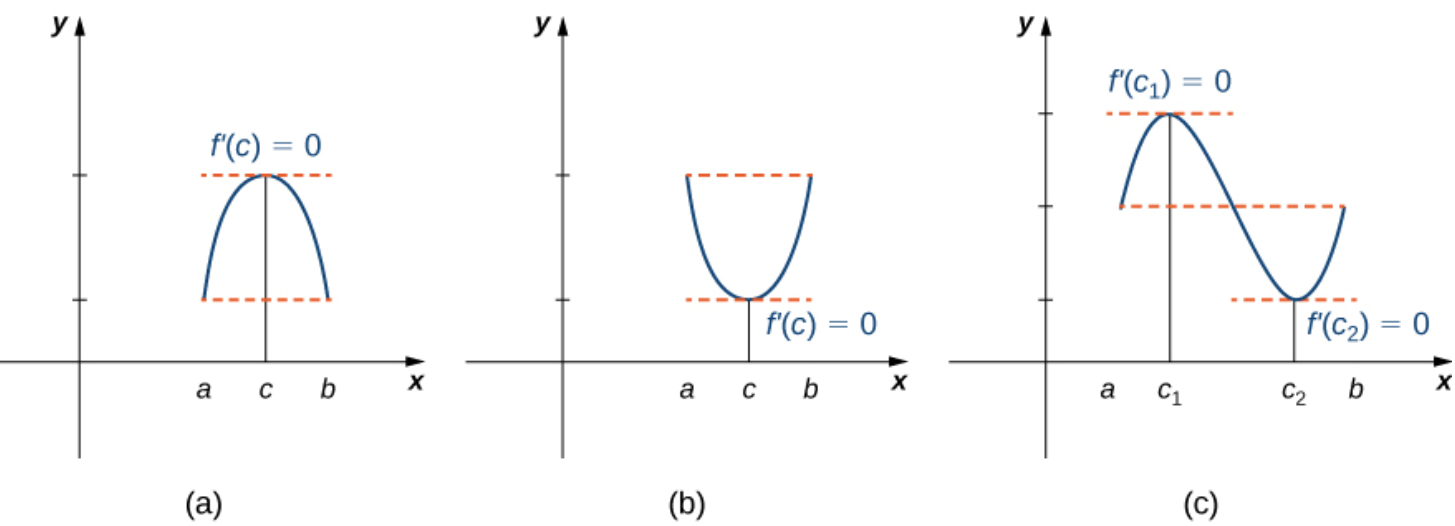
\includegraphics[scale=0.3]{img/image-20200323191523596.png}
\end{fullwidth}

\textbf{Skecth of Proof:} 
If the function is not a constant function, then the assumption of continuity implies that 
the function has a global extremum on $(a, b)$. Fermat's theorem implies the existence of $c$.

\textbf{Warning:} Differentiability is important. The following is a
counter-example.

  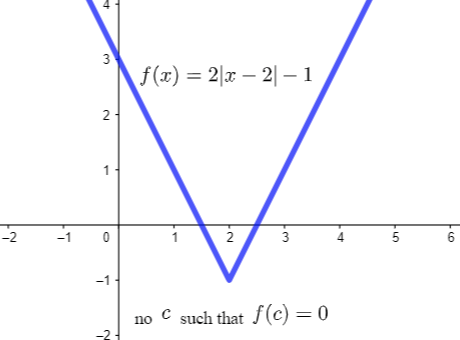
\includegraphics[scale=0.4]{img/image-20200323191152101.png}

\begin{example}

Verify that the function \(f(x)=x^2+4x-3\) satisfies the criteria stated
in Rolle's theorem and find all values \(c\) in the interval \((-7, 3)\)
at where \(f'(c)=0\).

\end{example}
\vspace*{6\baselineskip}

\begin{example}

Verify that the function \(f(x)=\sin x\) satisfies the criteria stated
in Rolle's theorem and find all values \(c\) in the interval
\((-\pi, \pi)\) at where \(f'(c)=0\).

\end{example}
\vspace*{6\baselineskip}

\hypertarget{mean-value-theorem-1}{%
\subsection{Mean Value Theorem}\label{mean-value-theorem-1}}

\begin{theorem}

Let \(f\) be a function continuous over a closed interval \([a,b]\) and
differentiable over the open interval \((a,b)\). Then exists at least
one value \(c\) in \((a,b)\) such that \[f'(c)=\frac{f(b)-f(a)}{b-a}.\]
\begin{fullwidth}
  \centering
  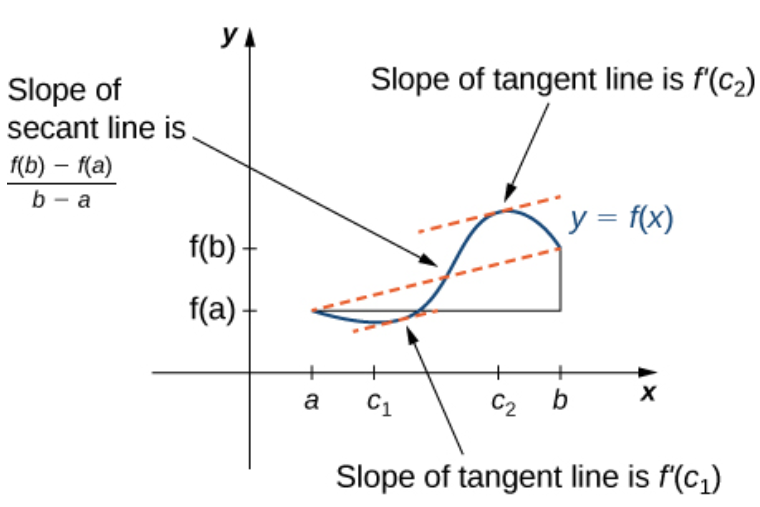
\includegraphics[scale=0.4]{img/image-20200323192552917.png}
\end{fullwidth}

\end{theorem}

To prove the theorem, let
\(g(x)=f(x) - [\frac{f(b) - f(a)}{b - a}(x - a)+f(a)]\), then apply Rolle's
theorem.

\begin{example}

Verify the function \(f(x)=\sqrt{x}\) defined over the interval
\([0,9]\) satisfies the condition of the Mean Value Theorem, and show
that there exists a value \(c\) in \((0,9)\) such that \(f'(c)\) is
equal to the slope of the secant line passing through \((0,f(0))\) and
\((9,f(9))\). Find these values \(c\) guaranteed by the Mean Value
Theorem.

\end{example}
\vspace*{6\baselineskip}

\begin{example}

Suppose that \(f(0)=-1\) and \(f'(x)>2\) for all values of \(x\) in
\([-2, 5]\). How small can \(f(5)\) possibly be?

\end{example}
\vspace*{6\baselineskip}

\hypertarget{corollaries-of-the-mean-value-theorem}{%
\subsection{Corollaries of the Mean Value
Theorem}\label{corollaries-of-the-mean-value-theorem}}

\begin{corollary}

Let \(f\) be a function differentiable over an interval \((a, b)\). If
\(f'(x)=0\) for all \(x\) in \((a, b)\), then \(f(x)=c\) for all \(x\)
in \((a, b)\), where \(c\) is a constant.

\end{corollary}

\begin{corollary}

Let \(f\) and \(g\) be two functions differentiable over an interval
\((a, b)\). If \(f'(x)=g'(x)\) for all \(x\) in \((a, b)\), then
\(f(x)=g(x)+c\) for all \(x\) in \((a, b)\), where \(c\) is a constant.

\end{corollary}

\begin{corollary}

Let \(f\) be a function continuous over the closed interval \([a,b]\)
and differentiable over the open interval \((a,b)\).

\begin{itemize}[sepno]
\item
  If \(f'(x)>0\) for all \(x\) in \((a, b)\), then \(f\) is increasing
  over \([a, b]\).
\item
  If \(f'(x)<0\) for all \(x\) in \((a, b)\), then \(f\) is decreasing
  over \([a, b]\).
\end{itemize}

\end{corollary}

\begin{example}

Show that the equation \(2x-\cos x=0\) has exactly one real root.

\end{example}
\vspace*{6\baselineskip}

\subsection{Practice}

\begin{exercise}

Verify that the function \(f(x)=\cos^2x\) satisfies the criteria stated
in Rolle's theorem and find all values \(c\) in the interval
\((-\pi, \pi)\) at where \(f'(c)=0\).

\end{exercise}
\vspace*{6\baselineskip}

\begin{exercise}

Suppose that \(f(-1)=2\) and \(f'(x)<3\) for all values of \(x\) less
that 6. How large can \(f(x)\) possibly be over the interval $[-1, 6]$?

\end{exercise}
\vspace*{6\baselineskip}

\begin{exercise}

Show that the equation \(x^2 + \cos x - 2=0\) has exactly one real root.

\end{exercise}

